\documentclass[screen]{beamer}
\usepackage[T1]{fontenc}
\usepackage[latin1]{inputenc}



% Bruk NTNU-temaet for beamer (her i bokmålvariant), alternativer er
% ntnunynorsk og ntnuenglish.
\usetheme{ntnuenglish}
 
% Angi tittelen, vi gir også en kortere variant som brukes nederst på
% hver slide:
\title[Mathematical Modelling]%
{Modelling of a neurotransmission}

% Denne kan du også bruke hvis det passer seg:
%\subtitle{Valgfri undertittel}

% Angir foredragsholder, også en (valgfri) kortversjon i
% hakeparanteser først som kommer nederst på hver slide:
\author[Group 9]{Group 9}

% Institusjon. Bruk gjerne disse slik det passer best med det du vil
% ha.  Valgfri kortversjon her også
\institute[NTNU]{Mathematical Modelling}

% Datoen blir også trykket på forsida. 
\date{14. November 2014}
%\date{} % Bruk denne hvis du ikke vil ha noe dato på forsida.

% Fra her av begynner selve dokumentet
\begin{document}
\setbeamertemplate{itemize items}[circle]

% Siden NTNU-malen har en annen bakgrunn på forsida, må dette gjøres
% i en egen kommando, ikke på vanlig beamer-måte:
\ntnutitlepage

% Her begynner første slide/frame, (nummer to etter forsida). 


\begin{frame}
\begin{columns}
    \begin{column}{.5\linewidth}
      \begin{block}{Modelling equations}
         \begin{align*}
         \frac{dc}{dt} &= \kappa \nabla^2 c \\
           \frac{dc}{dt} &= -k_1 c P^R + k_2 (1-P^R) \\
           \frac{dP^R}{dt} &=  -k_1 c P^R + k_2 (1-P^R)
         \end{align*}
      \end{block}
    \end{column}
    \begin{column}{.5\linewidth}
        \begin{figure}
  		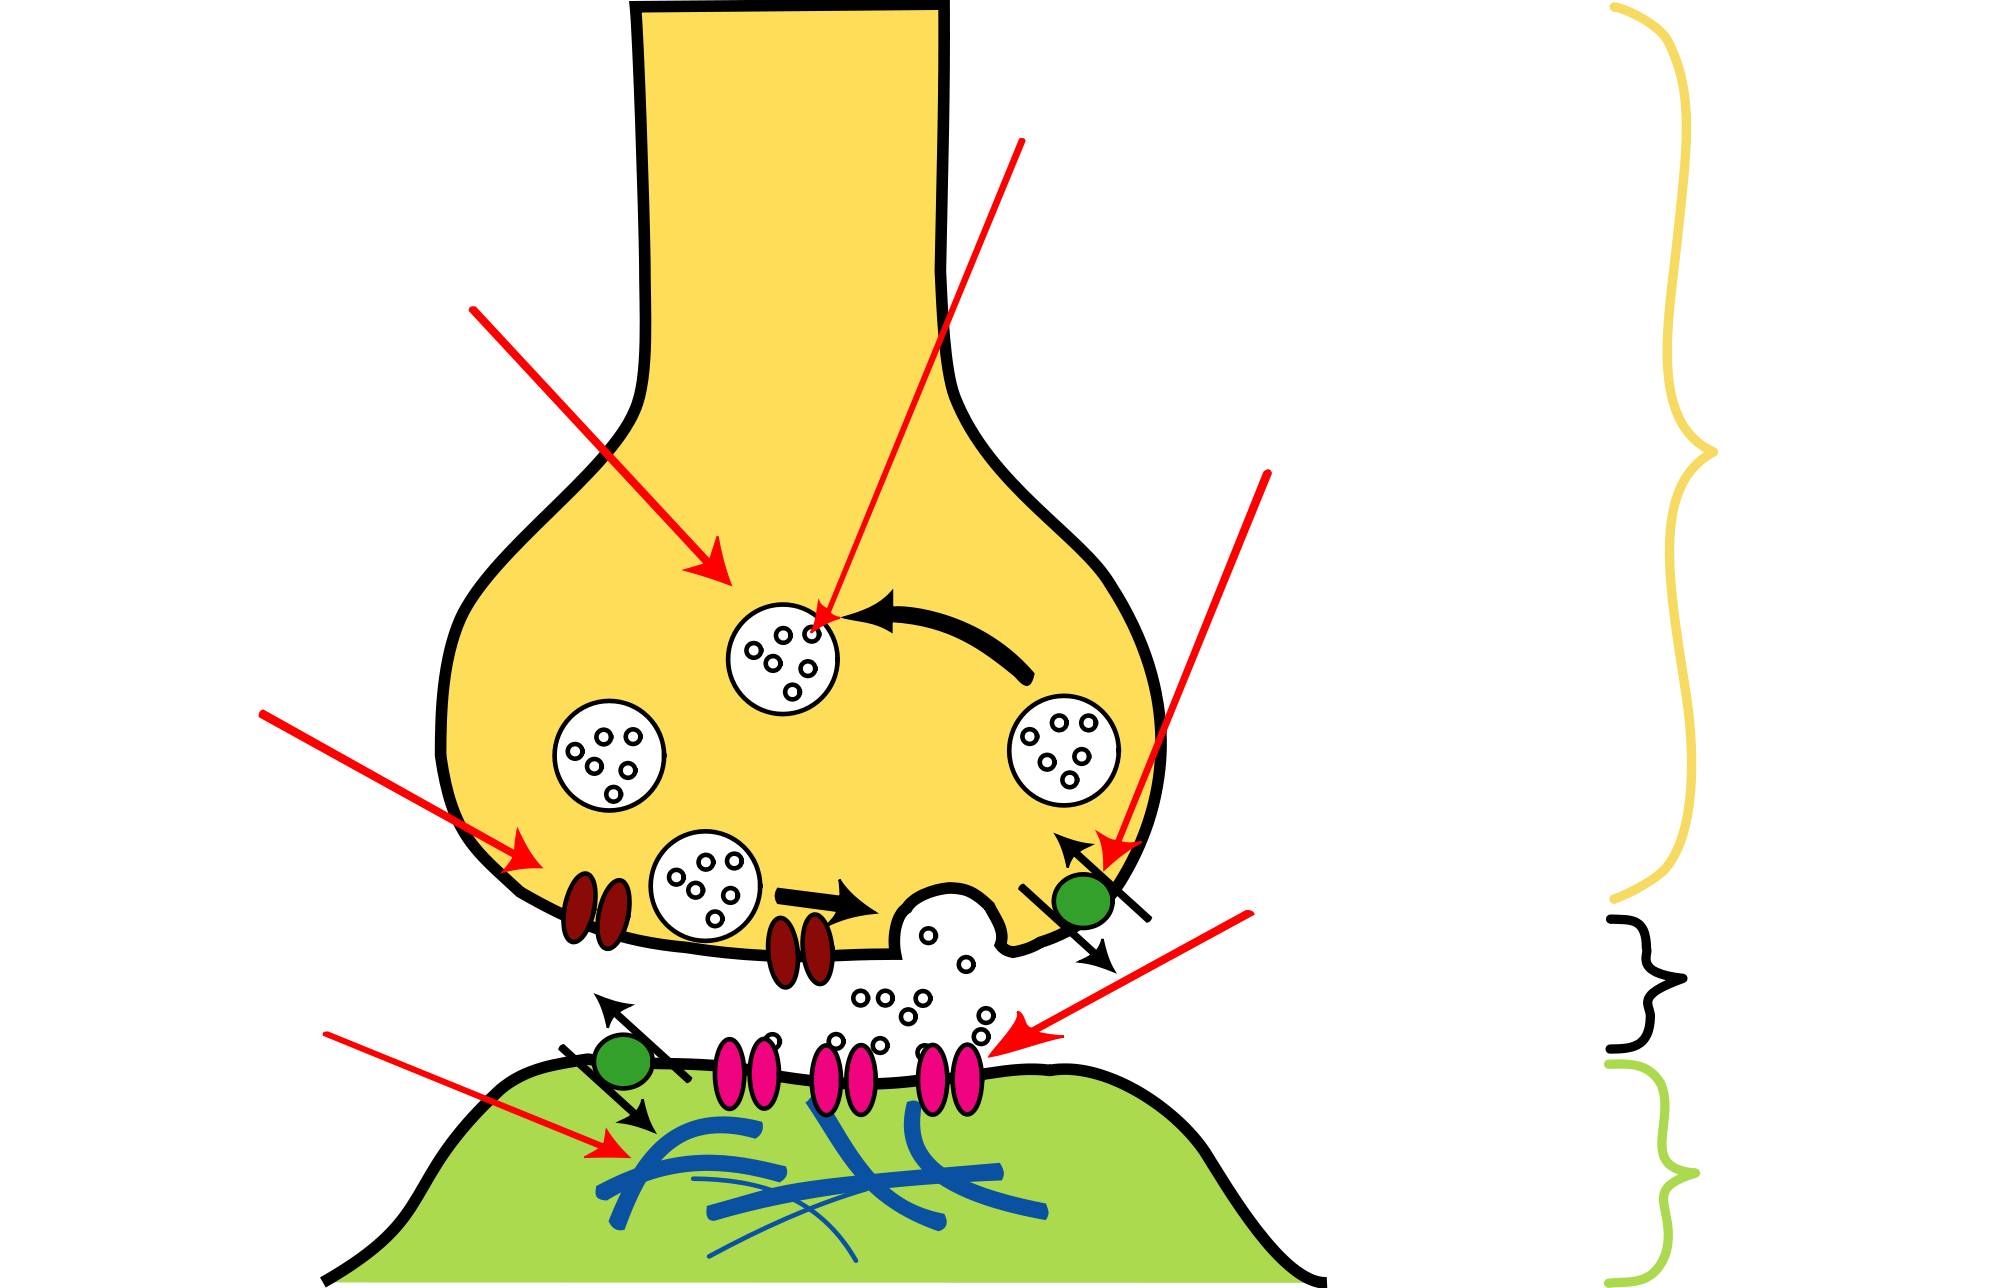
\includegraphics[scale=0.1]{synapse.png}
  		\end{figure}	
  		\tiny http://en.wikipedia.org/wiki/Chemical\_synapse\# mediaviewer/File:Synapse\_Illustration\_ unlabeled.svg
  		
    \end{column}
  \end{columns}
\end{frame}


\begin{frame}
  \frametitle{1D Model}
   \begin{figure}
   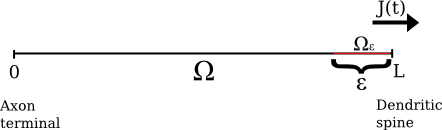
\includegraphics[scale=0.7]{model_1d.png}
  \end{figure}
\end{frame}



\begin{frame}
  \frametitle{1D distribution over time}
	
   \begin{figure}
   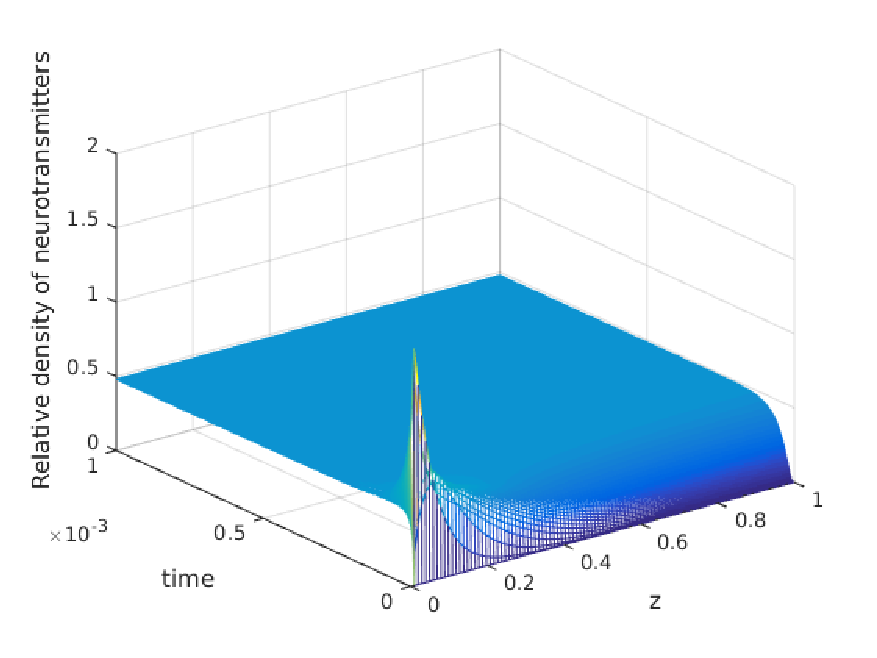
\includegraphics[scale=0.6]{1dmodel_plot-crop}
  \end{figure}
  
\end{frame}



\begin{frame}
	\frametitle{1D Model with glia cells}
	\begin{figure}
	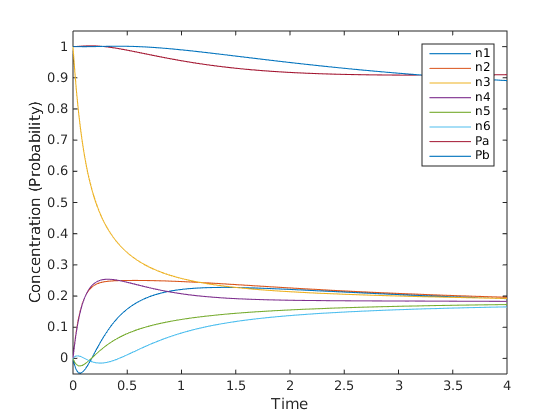
\includegraphics[scale=0.6]{1dodeLabels}
	\end{figure}
\end{frame}


\begin{frame}
	\frametitle{2D Model}
%	\begin{columns}
%    \begin{column}{.39\linewidth}
%    		\begin{itemize}
%    		\item Neglecting height in synaptic cleft
%    		\item Look at diffusion on a square
%    		\end{itemize}
%         
%    \end{column}
%    \begin{column}{.5\linewidth}
%        \begin{figure}
%  		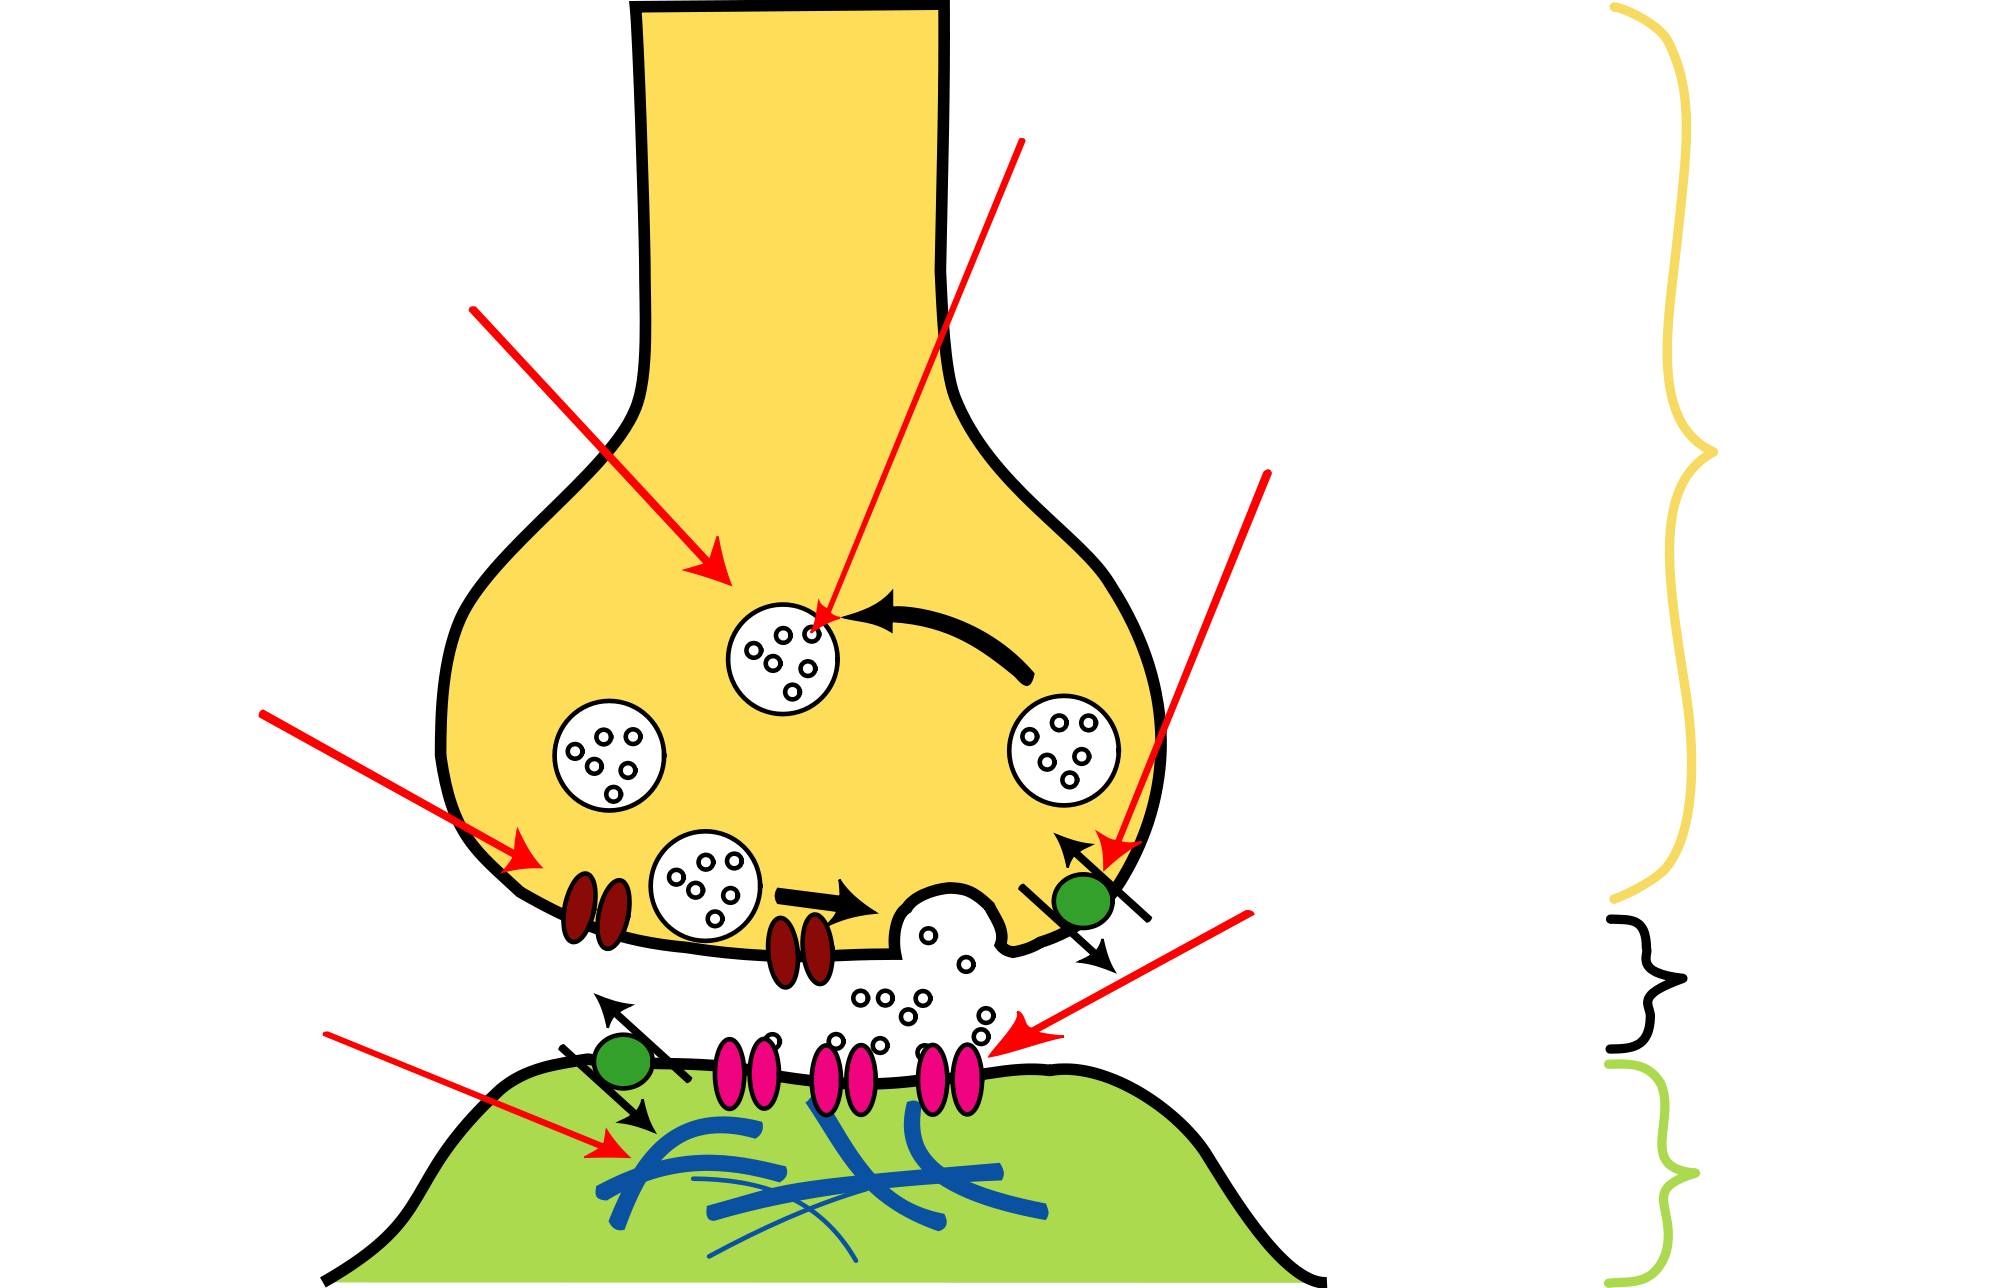
\includegraphics[scale=0.1]{synapse.png}
%  		\end{figure}	
%  		
%    \end{column}
%  \end{columns}
\begin{columns}
    \begin{column}{.5\linewidth}
        \begin{figure}
  		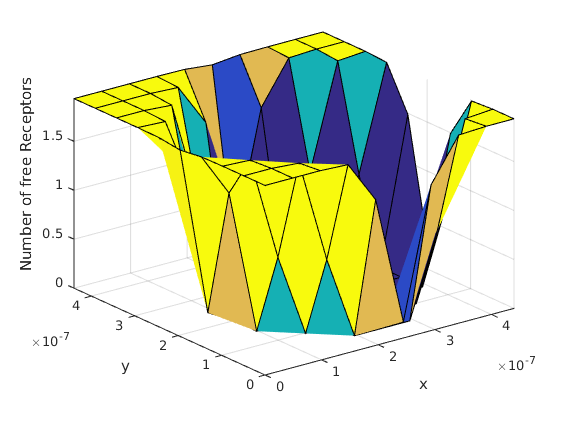
\includegraphics[scale=0.25]{receptordensity5ms}
  		\end{figure}
  		\begin{figure}
  		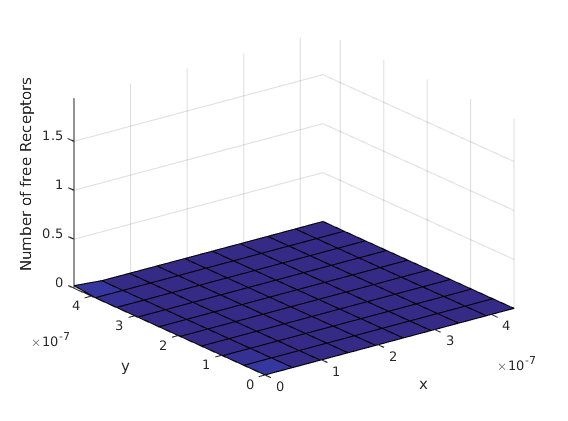
\includegraphics[scale=0.25]{receptordensity}
  		\end{figure}
    \end{column}
    \begin{column}{.5\linewidth}
        \begin{figure}
  		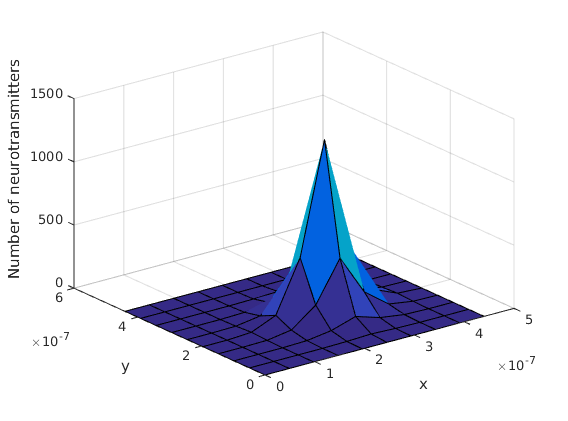
\includegraphics[scale=0.25]{distneurottansmitters5ms}
  		\end{figure}
  		\begin{figure}
  		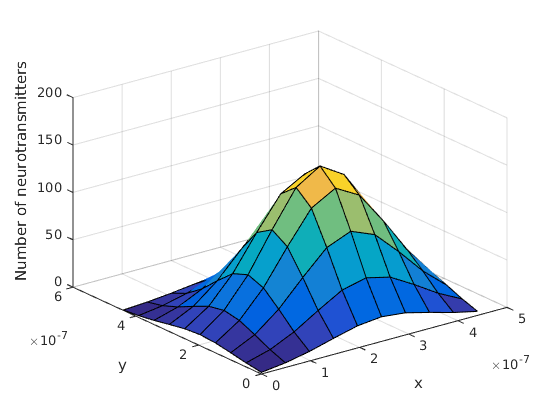
\includegraphics[scale=0.25]{distneurottansmitters}
  		\end{figure}
    \end{column}
  \end{columns}
%\begin{figure}[ht]
%    \centering
%    \begin{subfigure}[b]{0.45\textwidth}
%        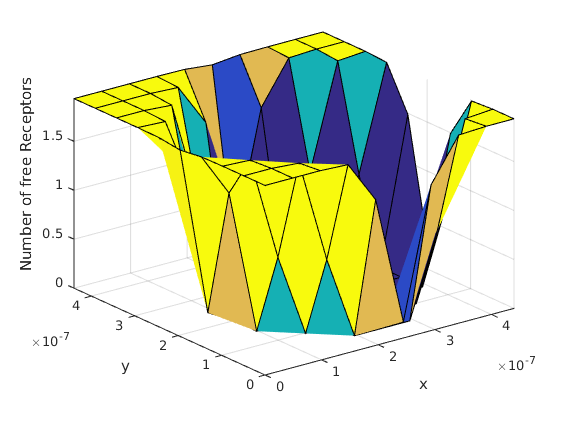
\includegraphics[width=\textwidth]{receptordensity5ms}
%        \caption{Distribution of free receptors at 5 ms.}
%    \end{subfigure}
%    ~ 
%    \begin{subfigure}[b]{0.45\textwidth}
%        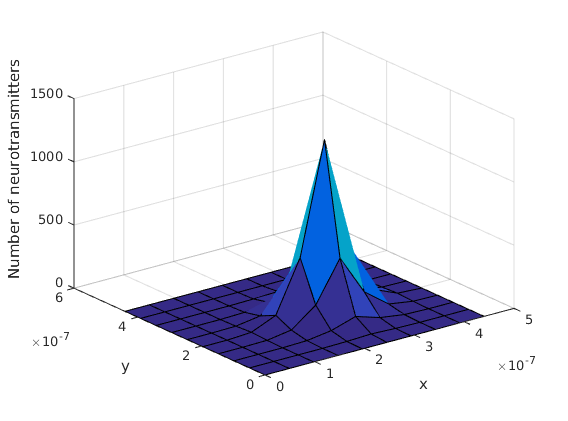
\includegraphics[width=\textwidth]{distneurottansmitters5ms}
%        \caption{Distribution of neurotransmitters at 5 ms.}
%    \end{subfigure}
%
%    \begin{subfigure}[b]{0.45\textwidth}
%        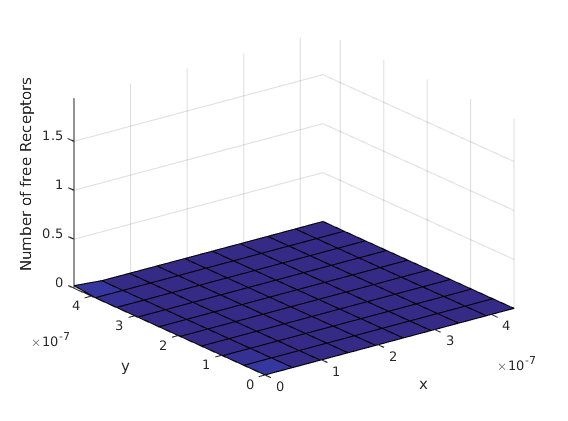
\includegraphics[width=\textwidth]{receptordensity}
%        \caption{Distribution of free receptors at signal time.}
%   %     \label{fig:receptordensitysignaltime}
%    \end{figure}
%   % ~
%    \begin{subfigure}[b]{0.45\textwidth}
%        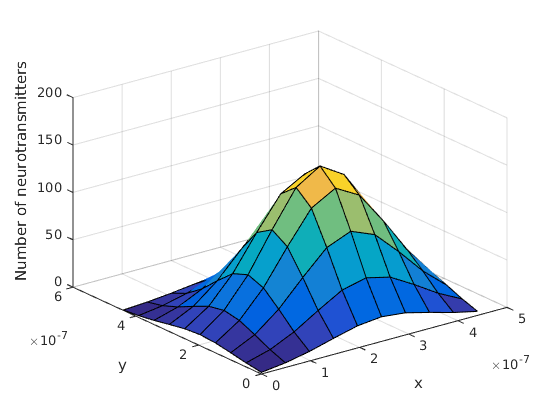
\includegraphics[width=\textwidth]{distneurottansmitters}
%   %     \caption{Distribution of neurotransmitters at signal time.}
%      %  \label{fig:concentrationOfReceptors2d}
%    \end{subfigure}    
    
  %  \caption{Simulation of the synaptic cleft at different times. This model is in 2 dimensions, ignoring height. In (a) and (c) the $z$-axis represents the number of free receptors. In (b) and (d) it represents the number of neurotransmitters.  Signaling time is 33.8 ms.}
%\end{figure}
\end{frame}


\begin{frame}
	\frametitle{3D Monte Carlo simulation}
\begin{columns}
    \begin{column}{.5\linewidth}
        \begin{figure}
  		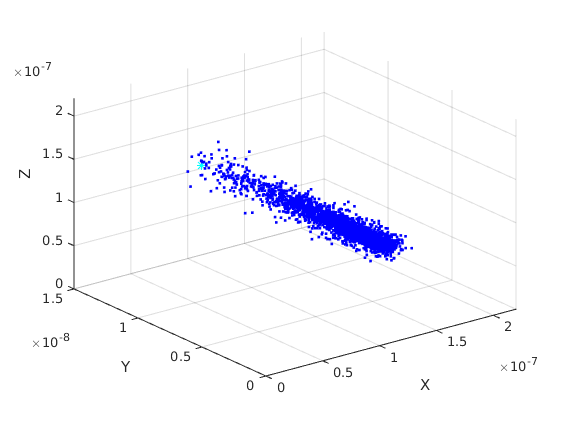
\includegraphics[scale=0.25]{sim01}
  		\end{figure}
  		\begin{figure}
  		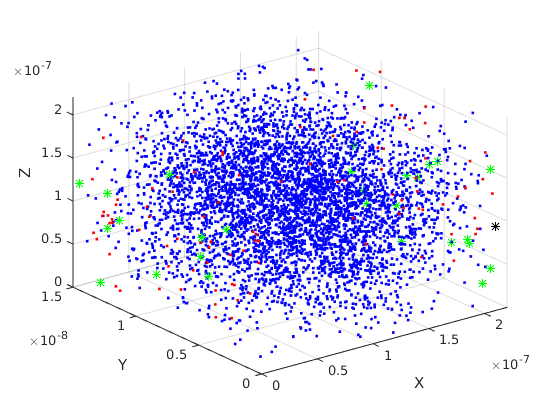
\includegraphics[scale=0.25]{sim03}
  		\end{figure}
    \end{column}
    \begin{column}{.5\linewidth}
        \begin{figure}
  		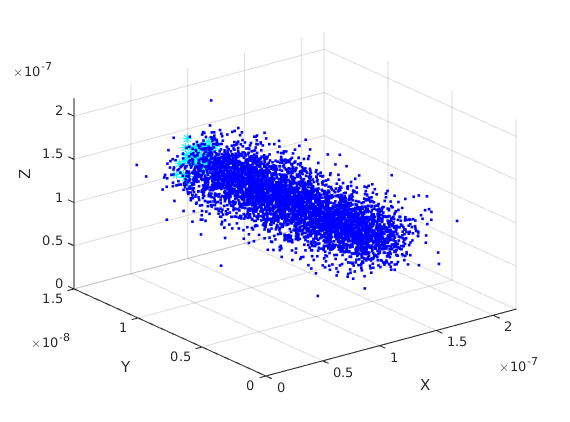
\includegraphics[scale=0.25]{sim02}
  		\end{figure}
  		\begin{figure}
  		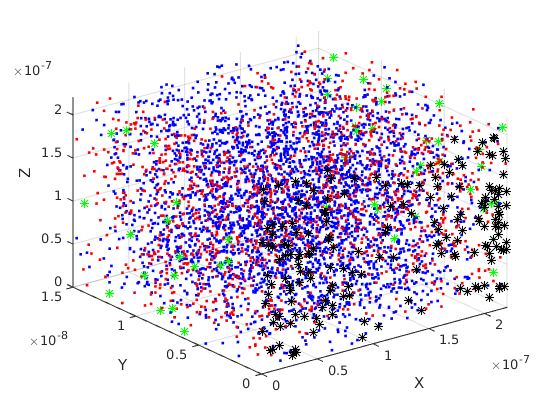
\includegraphics[scale=0.25]{sim04}
  		\end{figure}
    \end{column}
  \end{columns}
\end{frame}


\end{document}